\chapter{Z Tanım Bölgesinde PI Kontrolör Tasarımı}
Örnek sistem
\begin{equation}
    G(s)=\frac{1}{s+2}
\end{equation}
z tanım bölgesinde $T=0.2$ olmak üzere
\begin{equation}
    G(z)=\frac{0.1648}{z-0.6703}
\end{equation}
olarak elde edilmektedir. Yerleşme zamanı $t_s=2$ ve aşım $\%10$ isterleri verilmiştir. Bu durumda $\zeta=0.591$ ve $w_n=6.7664$ seçilir. Seçilen sönüm oranı ve doğal frekans ile baskın kutuplar
\begin{equation}
    s_{1,2}=-4 \pm 5.4575i
\end{equation}
şeklinde hesaplanır. $z=e^{sT}$ ifadesi ile z tanım bölgesinde kutuplar
\begin{equation}
    z_{1,2}=0.2072 \pm 0.3987i
\end{equation}
ve kutuplardan oluşturulacak polinom
\begin{equation}
    p(z)=z^2-0.4144 z+0.2019
\end{equation}
olarak hesaplanır. PI kontrolörü 
\begin{equation}
\begin{split}
    F(z)&=K_p+\frac{K_iz}{z-1}\\
    &=\frac{(K_p+K_i)z-K_p}{z-1}
\end{split}
\end{equation}
olarak tanımlanmıştır. Kapalı çevrim transfer fonksiyonu 
\begin{equation}
    \begin{split}
        T(z)&=\frac{F(z)G(z)}{1+F(z)G(z)}\\
        &=\frac{\frac{(K_p+K_i)z-K_p}{z-1}\frac{0.1648}{z-0.6703}}{1+\frac{(K_p+K_i)z-K_p}{z-1}\frac{0.1648}{z-0.6703}}\\
        &=\frac{0.1648(K_p+K_i)z-0.1648K_p}{z^2+(0.1648(K_p+K_i)-1.6703)z+0.6703-0.1648K_p}
    \end{split}
\end{equation}
şeklindedir. Tasarım problemi
\begin{equation}
    \begin{split}
       0.1648(K_p+K_i)-1.6703&=-0.4144\\
       0.6703-0.1648K_p&=0.2019
    \end{split}
\end{equation}
ve çözüm ise $K_p=2.8423$ ve $K_i=4.7784$ şeklindedir. Bu durumda PI kontrolör
\begin{equation}
        F(z)=\frac{7.621 z - 2.842}{z-1}
\end{equation}
ve kapalı çevrim transfer fonksiyonu
\begin{equation}
\begin{split}
    T(z)&=\frac{1.256 z - 0.4685}{z^2 - 0.4141 z + 0.2018}\\
    &=\frac{1.2562 (z-0.373)}{z^2 - 0.4141 z + 0.2018}\\
\end{split}
\end{equation}
olarak elde edilir.
\begin{figure}[!htb]
    \centering
    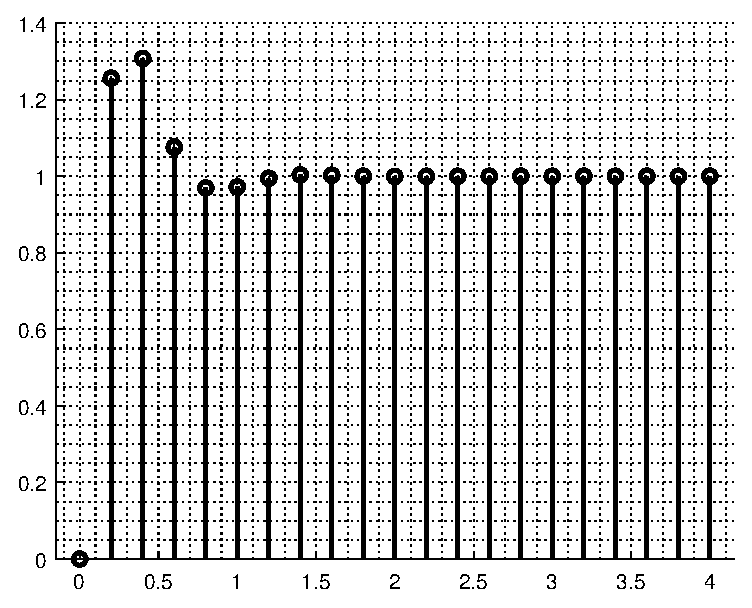
\includegraphics[width=0.75\textwidth]{img/lec9_step1}
    \caption{PI kontrol için kapalı çevrim basamak yanıtı}
    \label{fig:lec9_step1}
\end{figure}

Kapalı çevrim basamak yanıtı için yerleşme zamanı $t_s=1.2\,s$ ve aşım $\%30.79$'dur. İsterler tam sağlanmasa da yerleşme zamanı kabul edilebilir elde edilmiştir. 